\textcolor{red}{\section{Compare Performance on Yolov5 Segment and Dataset Offter Finger Knuckle}}

\textcolor{red}{This section aim to compare quality of finger knuckle between Yolov5 segmented and dataset offered. Because the segmented finger knuckle on the 3D Finger Knuckle Dataset already have high quality, I mainly test on the Index Finger Knuckle of Hand Dorsal Dataset and the Finger Knuckle Dataset V3 (with deformable).}

\begin{figure}[H]
	\centering
	\begin{subfigure}[b]{0.8\linewidth}
		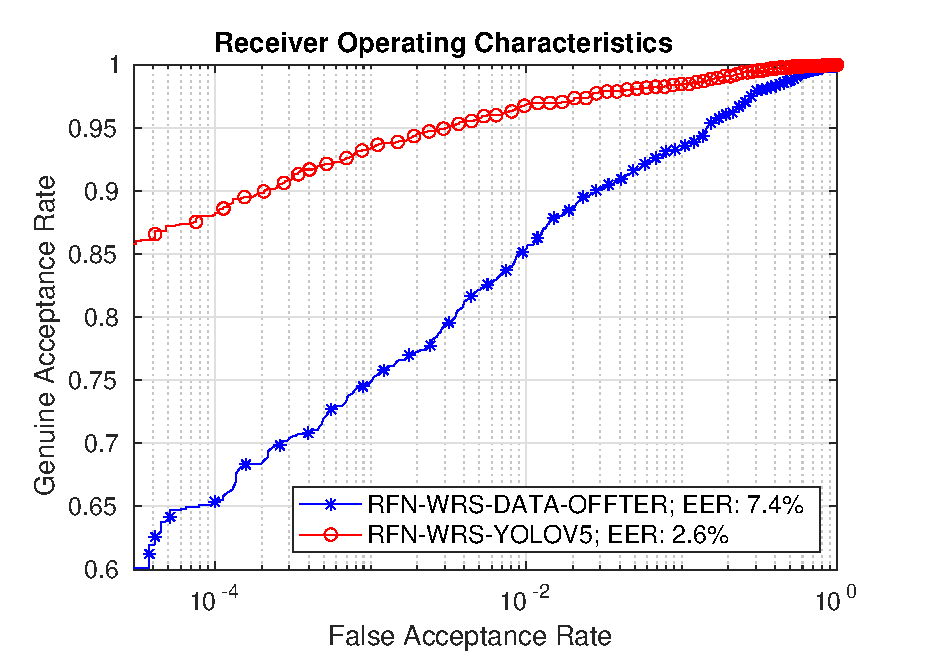
\includegraphics[width=\linewidth]{Figures/yolov5vsdata/fkv3-roc_compare_new.eps}
        \caption{Compare performance on the Finger Knucle V3 Dataset (with deformable)}
	\end{subfigure}
	\begin{subfigure}[b]{0.8\linewidth}
		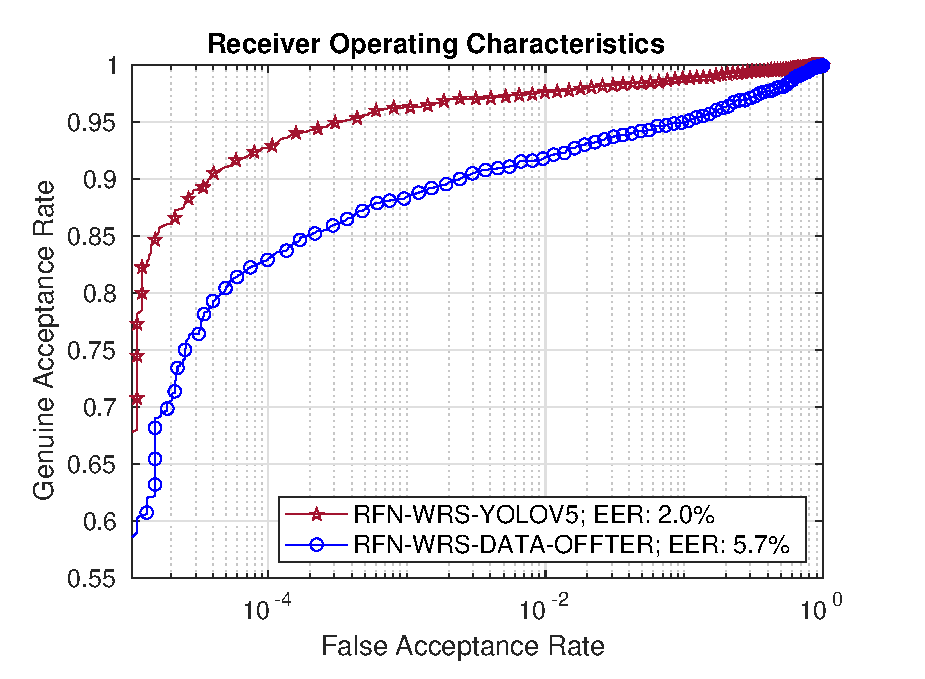
\includegraphics[width=\linewidth]{Figures/yolov5vsdata/hd-roc_compare_new.eps}
        \caption{Compare performance on the Index Finer Knukle of Hand Dorsal Dataset}
	\end{subfigure}
    \caption{}
\end{figure}

\textcolor{red}{From the above figures, we can clearly get the conclusion that quality of segmented finger knuckle of YOLOV5 is better than the segmented finger knuckle of dataset based on the same model. Especially on the Finger Knuckle V3 Dataset, the EER value can drop from $7.4\%$ to $2.6\%$.}

\vspace{10pt}

\textcolor{red}{Because in the previous experiments, except for Finger Knuckle V3 and 3D Finger Knuckle Dataset, other datasets were segmented using the YOLOV5 model. But with Yolov5 segmented finger knuckle, the RFNet performance is slightly higer than the local feature descriptors based on key points matching \cite{kumar2020contactless}, and performance higher than the paper \cite{kumar2019toward}. If we want to compare different method performance, I think we should use same dataset. In this kind of situation, the method of \cite{kumar2020contactless} maybe will ger higer performance on the segmented finger knuckle by YOLOV5.}